\documentclass[aspectratio=169]{beamer}
\usepackage[utf8]{inputenc}
\usepackage[T1]{fontenc}
\usepackage[brazil]{babel}
\usepackage{ragged2e}
\usepackage{booktabs}
\usepackage{verbatim}
\usetheme{AnnArbor}
\usecolortheme{orchid}
\usefonttheme[onlymath]{serif}
\usepackage{listings}
\usepackage{colortbl}
\usepackage{array}

\newcolumntype{C}[0]{>{\centering\arraybackslash}p{0.4cm}}

\lstset{language=C++,
	backgroundcolor=\color{green!10},
	basicstyle=\ttfamily,
	keywordstyle=\color{blue}\ttfamily,
	stringstyle=\color{red}\ttfamily,
	commentstyle=\color{brown}\ttfamily,
	morecomment=[l][\color{magenta}]{\#},
	literate=
	{á}{{\'a}}1
	{à}{{\`a}}1
	{ã}{{\~a}}1
	{â}{{\^a}}1
	{é}{{\'e}}1
	{ê}{{\^e}}1
	{í}{{\'i}}1
	{ó}{{\'o}}1
	{õ}{{\~o}}1
	{ú}{{\'u}}1
	{ü}{{\"u}}1
	{ç}{{\c{c}}}1
	{Á}{{\'A}}1
	{À}{{\`A}}1
	{Ã}{{\~A}}1
	{Â}{{\^A}}1
	{É}{{\'E}}1
	{Ê}{{\^E}}1
	{Í}{{\'I}}1
	{Ó}{{\'O}}1
	{Õ}{{\~O}}1
	{Ú}{{\'U}}1
	{Ü}{{\"U}}1
	{Ç}{{\c{C}}}1
}

\AtBeginSection[]{
  \begin{frame}
  \vfill
  \centering
  \begin{beamercolorbox}[sep=8pt,center,shadow=true,rounded=true]{title}
    \usebeamerfont{title}\insertsectionhead\par%
  \end{beamercolorbox}
  \vfill
  \end{frame}
}

\title[\sc{Estruturas Lineares}]{Estruturas Lineares}
\author[Roland Teodorowitsch]{Roland Teodorowitsch}
\institute[ALEST I - EP - PUCRS]{Algoritmos e Estruturas de Dados I - Escola Politécnica - PUCRS}
\date{25 de setembro de 2024}

\begin{document}

\justifying

%-------------------------------------------------------
\begin{frame}
	\titlepage
\end{frame}

%=======================================================
\section{Introdução}

%-------------------------------------------------------
\begin{frame}\frametitle{Leitura(s) Recomendada(s)}

\begin{columns}[T]
\begin{column}{0.15\linewidth}
\vspace{-3mm}
\begin{figure}[h]
	\centering
	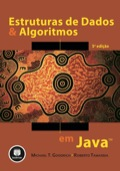
\includegraphics[height=0.3\paperheight]{imagens/livro_goodrich.jpg}
\end{figure}
\end{column}
%\vspace{3mm}
\begin{column}{0.85\linewidth}
\tiny{\textbf{Seções 3.2 (Listas simplesmente encadeadas), 3.3 (Listas duplamente encadeadas), 6.1 (Listas arranjo), 6.2 (Listas de nodos), 6.4 (Os TADs de lista e o \emph{framework} de coleções)}\\
~}\\
\scriptsize{GOODRICH, Michael T.; TAMASSIA, Roberto. \textbf{Estruturas de dados e algoritmos em Java}. Tradução: Bernardo Copstein. 5. ed. Porto Alegre: Bookman, 2013. xxii, 713 p. E-book. ISBN 9788582600191. Tradução de: Data Structures and Algorithms in Java, 5th Edition. Disponível em: \textless{}\url{https://integrada.minhabiblioteca.com.br/\#/books/9788582600191/}\textgreater{}. Acesso em: 01 ago. 2023.}
\end{column}
\end{columns}

\end{frame}

%=======================================================
\section{Tipos Abstratos de Dados}

%-------------------------------------------------------
\begin{frame}\frametitle{Abordagem OO}
\begin{itemize}
	\item Princípios da abordagem OO
	\begin{itemize}
		\item \textbf{Abstração}: representação de um objeto do mundo real, ``abstraindo-se'' os detalhes desnecessários, de forma que o objeto possa ser utilizado sem se preocupar com como ele foi implementado
		\item \textbf{Encapsulamento}: detalhes da implementação ficam escondidos e a manipulação dos dados acontede através de uma interface pública
		\item \textbf{Modularidade}: vários componentes que interagem
	\end{itemize}
	\item Abstração, Encapsulamento, Herança e Polimorfismo são considerados os 4 pilares da POO
\end{itemize}
\end{frame}

%-------------------------------------------------------
\begin{frame}\frametitle{Tipos Abstratos de Dados}
\begin{itemize}
	\item A aplicação de abstração ao projeto de estruturas de dados nos leva a \textbf{Tipos Abstratos de Dados (TAD)}
	\item TAD
	\begin{itemize}
		\item É uma especificação de um conjunto de dados e operações que podem ser executadas sobre esses dados
		\item Modelo matemático de estruturas de dados que especifica
		\begin{itemize}
			\item O tipo dos dados armazenados
			\item As operações definidas sobre esses dados
			\item Os tipos dos parâmetros dessas operações
		\end{itemize}
	\end{itemize}
	\item A separação de especificação e implementação permite usar um TAD sem conhecer nada sobre a sua implementação
	\begin{itemize}
		\item Assim, um TAD pode ter mais de uma implementação
	\end{itemize}
\end{itemize}
\end{frame}

%-------------------------------------------------------
\begin{frame}\frametitle{TAD}
\begin{itemize}
	\item Usa ``encapsulamento''
	\item Princípio: esconder detalhes de representação e direcionar o acesso aos objetos abstratos por meio de operações
	\item A representação fica protegida contra qualquer tentativa de manipulá-la diretamente (só através das operações disponíveis)
	\item Define o que cada operação faz, mas não como o faz
\end{itemize}
\end{frame}

%-------------------------------------------------------
\begin{frame}\frametitle{Tipos Abstratos de Dados}
\begin{itemize}
	\item Resumindo, TAD é uma estrutura de programa que contém
	\begin{itemize}
		\item A especificação de uma estrutura de dados
		\item Um conjunto de operações que podem ser realizadas sobre os dados encapsulados
	\end{itemize}
	\item Exemplos de TADs
	\begin{itemize}
		\item Pilhas, Filas, Deques e Listas
	\end{itemize}
	\item Essas estruturas são classificadas como lineares
	\begin{itemize}
		\item Representam coleções de elementos linearmente organizados que oferecem métodos para inserir, acessar e remover elementos
		\item Têm a ordem interna de seus elementos definida pela forma como são feitas inserções e remoções na estrutura
		\item Costumam ter duas extremidades (esquerda e direita; frente e traseira; cabeça e cauda; ...)
	\end{itemize}
\end{itemize}
\end{frame}

%-------------------------------------------------------
\begin{frame}\frametitle{Estruturas Lineares}
\begin{itemize}
	\item \textbf{Lista}
	\begin{itemize}
		\item Organiza os dados de maneira ``sequencial'' (não necessariamente de forma física, mas sempre existe uma ordem lógica entre os elementos)
		\item Permite inserção, acesso e remoção de elementos
	\end{itemize}
	\item \textbf{Pilha}
	\begin{itemize}
		\item Usa a política \emph{LIFO -- Last In First Out} (o último elemento que entrou, é o primeiro a sair)
		\item Possui apenas uma entrada, chamada de topo, a partir da qual os dados entram e saem dela
	\end{itemize}
	\item \textbf{Fila}
	\begin{itemize}
		\item Usa a política \emph{FIFO -- First In First Out} (o primeiro elemento a entrar será o primeiro a sair)
		\item Os elementos entram por um lado (``cauda'' ou parte de trás) e saem por outro (``cabeça'' ou parte da frente)
	\end{itemize}
	\item \textbf{Deque} (\emph{Double-Ended QUEue})
	\begin{itemize}
		\item Os elementos entram e saem por qualquer uma das extremidades (cauda ou cabeça) da lista
	\end{itemize}
\end{itemize}
\end{frame}

%-------------------------------------------------------
\begin{frame}\frametitle{Estruturas Lineares}
\begin{itemize}
	\item Permitem representar um conjunto de dados de um mesmo tipo (com alguma afinidade) de forma a preservar a relação de ordem entre seus elementos
	\item Cada elemento da estrutura é chamado de nó, ou nodo.
	\item Uma estrutura linear é definida como:
	\begin{itemize}
		\item Um conjunto de $N$ nós, organizados de forma a refletir a posição relativa dos mesmos
		\item Se $N > 0$, os nós da estrutura serão $x_1$, $x_2$, ..., $x_N$, 
		\begin{itemize}
			\item $x_1$ é o primeiro nó
			\item Para $1 < k < N$, o nó $x_k$ é precedido pelo nó $x_{k-1}$ e seguido pelo nó $x_{k+1}$
			\item $x_N$ é o último nó
		\end{itemize}
		\item Quando $N = 0$, diz-se que a estrutura está vazia
	\end{itemize}
\end{itemize}
\end{frame}

%-------------------------------------------------------
\begin{frame}\frametitle{Exemplos de Estruturas Lineares}
\begin{itemize}
	\item Pessoas na fila de um caixa (ordem definida pela chegada e posição na fila)
	\item Pessoas na sala de espera de um consultório (ordem definida pela chegada)
	\item Conjunto de notas dos alunos de uma turma
	\item Itens no estoque de uma loja
	\item Palavras de um texto
	\item Letras de uma palavra
	\item Especificação de operações e operandos em uma expressão matemática
	\item Dias da semana
	\item Relação de compromissos
	\item Pilha de livros
	\item Cartas de um baralho
	\item etc.
\end{itemize}
\end{frame}

%-------------------------------------------------------
\begin{frame}[fragile]\frametitle{Alocação de Estruturas Lineares}
\begin{itemize}
	\item Estruturas lineares podem ser alocadas de forma:
	\begin{itemize}
		\item \textbf{Sequencial ou Contígua}\\Os nós, além de estarem em uma sequência lógica, também estão \textbf{fisicamente em sequência}
\begin{figure}[h]
	\centering
	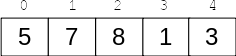
\includegraphics[height=0.10\paperheight]{imagens/vetor.png}
\end{figure}
		\item \textbf{Encadeada}\\Os nós são alocados dinamicamente e são ligados entre si, de forma que há uma sequência lógica, mas fisicamente os nós NÃO precisam estar contíguos
\begin{figure}[h]
	\centering
	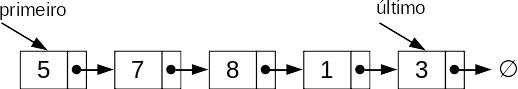
\includegraphics[height=0.15\paperheight]{imagens/lista_simplesmente_encadeada.png}
\end{figure}
	\end{itemize}
	\item Cada forma tem as suas vantagens e desvantagens
\end{itemize}
\end{frame}

%-------------------------------------------------------
\begin{frame}\frametitle{Alocação Sequencial ou Contígua de Estruturas Lineares}
\begin{itemize}
	\item Nós adjacentes na estrutura são armazenados em endereços contíguos na memória física e o tamanho da estrutura é fixo
	\item A implementação é feita com vetores (arranjos ou \emph{arrays}), que podem ser alocados de forma estática ou dinâmica
	\item Pode-se trabalhar com vetores parcialmente prenchidos
	\item O acesso é rápido
	\item NÃO é possível ter espaços vazios (não utilizados) no meio da estrutura (a não ser no final, para vetores parcialmente preenchidos)
	\item Inserção e Remoção de elementos no meio exige movimentação de elementos
	\item Para estruturas alocadas dinamicamente, pode-se: alocar um novo vetor, copiar os elementos do antigo para o novo, desalocar o antigo e passar a usar o novo -- mas isto pode ser custoso
\end{itemize}
\end{frame}
	
%-------------------------------------------------------
\begin{frame}[fragile]\frametitle{Alocação Sequencial ou Contígua de Estruturas Lineares (vetores.cpp)}
\lstinputlisting[basicstyle=\ttfamily\tiny]{src/vetores.cpp}
\end{frame}

%-------------------------------------------------------
\begin{frame}[fragile]\frametitle{Alocação Sequencial ou Contígua de Estruturas Lineares (vetores2.cpp)}
\lstinputlisting[basicstyle=\ttfamily\tiny]{src/vetores2.cpp}
\end{frame}

%-------------------------------------------------------
\begin{frame}\frametitle{Alocação Encadeada de Estruturas Lineares}
\begin{itemize}
	\item Os elementos da estrutura seguem uma ordem lógica, mas \textbf{NÃO estão necessariamente armazenados sequencialmente na memória}
	\item A relação lógica de ordem é implementada através de uma ligação (referência ou armazenamento de endereço) entre os nodos
	\item Estruturas lineares encadeadas são chamadas de \textbf{listas encadeadas}, sendo que cada nodo pode armazenar uma referência para o próximo elemento (lista simplesmente encadeada)
\begin{figure}[h]
	\centering
	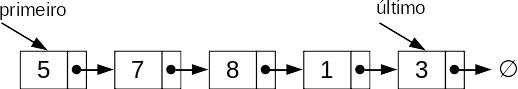
\includegraphics[height=0.15\paperheight]{imagens/lista_simplesmente_encadeada.png}
\end{figure}
	\item Ou para o elemento anterior e para o próximo elemento (lista duplamente encadeada)
\begin{figure}[h]
	\centering
	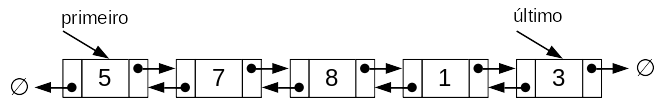
\includegraphics[height=0.16\paperheight]{imagens/lista_duplamente_encadeada.png}
\end{figure}
	\item A estrutura pode aumentar e diminuir em tempo de execução
\end{itemize}
\end{frame}

%-------------------------------------------------------
\begin{frame}\frametitle{Alocação Encadeada de Estruturas Lineares}
\begin{itemize}
	\item Quando for necessário inserir um elemento na estrutura, deve-se:
	\begin{itemize}
		\item Alocar um novo nodo
		\item Preencher as informações no nodo
		\item Inserir o novo nodo em determinada posição da estrutura (o que exige ajustes em alguns encadeamentos)
	\end{itemize}
	\item Alocação encadeada será útil quando:
	\begin{itemize}
		\item Não é possível prever o número de entradas de dados em tempo de compilação
		\item For mais fácil aplicar determinada operação sobre a estrutura encadeada
	\end{itemize}
\end{itemize}
\end{frame}

%-------------------------------------------------------
\begin{frame}\frametitle{Operações Básicas sobre Estruturas Lineares}
\begin{itemize}
	\item Criação da estrutura
	\item Destruição da estrutura
	\item Inserção de um elemento na estrutura
	\item Remoção de um elemento da estrutura
	\item Acesso a um elemento da estrutura
	\item Alteração de um elemento da estrutura
	\item Combinação de duas ou mais estruturas
	\item Ordenação dos elementos da estrutura
	\item Cópia de uma estrutura
	\item Localização de um nodo através de alguma informação do nodo
\end{itemize}
\end{frame}

%=======================================================
\section{Pilha (\emph{Stack})}

%-------------------------------------------------------
\begin{frame}\frametitle{Pilha ou \emph{Stack}}
\begin{itemize}
	\item Usa a política \emph{LIFO -- Last In First Out} (o último elemento que entrou, é o primeiro a sair)
	\item Possui apenas uma entrada, chamada de topo, a partir da qual os dados são inseridos e removidos
\begin{figure}[h]
	\centering
	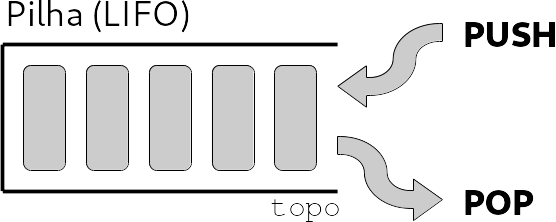
\includegraphics[height=0.3\paperheight]{imagens/pilha.png}
\end{figure}
\end{itemize}
\end{frame}

%-------------------------------------------------------
\begin{frame}\frametitle{Pilha: Implementações Possíveis}
\begin{itemize}
	\item \textbf{Arranjo}
\begin{figure}[h]
	\flushleft
	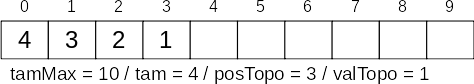
\includegraphics[height=0.15\paperheight]{imagens/pilha1.png}
\end{figure}
	\item \textbf{Lista Simplesmente Encadeada}
\begin{figure}[h]
	\flushleft
	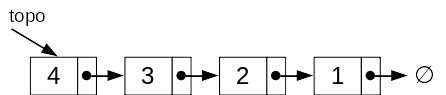
\includegraphics[height=0.15\paperheight]{imagens/pilha2.png}
\end{figure}
	\item \textbf{Lista Duplamente Encadeada}
\begin{figure}[h]
	\flushleft
	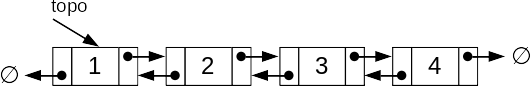
\includegraphics[height=0.15\paperheight]{imagens/pilha3.png}
\end{figure}
\end{itemize}
\end{frame}

%-------------------------------------------------------
\begin{frame}\frametitle{Aplicações que Usam Pilha}
\begin{itemize}
	\item Operações de edição de desfazer/refazer
	\item Histórico de visitação de páginas em navegadores \emph{web} (botão \emph{back})
	\item Cadeia de chamada de métodos em interpretadores e máquinas virtuais
	\item Auxiliar para implementação de outras estruturas de dados e algoritmos
	\item Implementação de compiladores
	\item Computação Gráfica (operações com matrizes)
	\item Manipulação de expressões aritméticas: infixada, pré-fixada, pós-fixada
\end{itemize}
\end{frame}

%-------------------------------------------------------
\begin{frame}\frametitle{Manipulação de Expressões Aritméticas}
\begin{itemize}
	\item Expressões aritméticas geralmente são representadas usando a notação infixada\\
		\texttt{2 + 3 * 4 = 14}\\
		\texttt{(2 + 3) * 4 = 20}
	\item Alternativa 1: Notação polonesa (pré-fixada)
	\begin{itemize}
		\item Proposta por Jan lukasiewiscz em 1920
		\item Permite escrever expressões aritméticas com precedência implícita
		\item Operador aparece antes dos operandos\\
			\texttt{+ 2 * 3 4}\\
			\texttt{* + 2 3 4}
	\end{itemize}
	\item Alternativa 2: Notação polonesa inversa (pós-fixada)
	\begin{itemize}
		\item Proposta por Charles Hamblin em 1950
		\item Também usa precedência implícita, porém o operandor aparece antes dos operandos\\
			\texttt{2 3 4 * +}\\
			\texttt{2 3 + 4 *}
	\end{itemize}
\end{itemize}
\end{frame}

%-------------------------------------------------------
\begin{frame}\frametitle{Exercício}
Converta as seguintes expressões na forma infixada para as formas pré-fixada e pós-fixada:
\begin{enumerate}
	\item	Infixada: \texttt{(1-2)*(3+4)}\\
		Pré-fixada: \\
		Pós-fixada: \\
	\item	Infixada: \texttt{(2 + 4)/(3 -1)}\\
		Pré-fixada: \\
		Pós-fixada: \\
	\item	Infixada: \texttt{(2+4)/(3-1)*4}\\
		Pré-fixada: \\
		Pós-fixada: \\
\end{enumerate}
\end{frame}

%-------------------------------------------------------
\begin{frame}\frametitle{Exercício (Resposta)}
Converta as seguintes expressões na forma infixada para as formas pré-fixada e pós-fixada:
\begin{enumerate}
	\item	Infixada: \texttt{(1-2)*(3+4)}\\
		Pré-fixada: \texttt{* - 1 2 + 3 4}\\
		Pós-fixada: \texttt{1 2 - 3 4 + *}\\
	\item	Infixada: \texttt{(2 + 4)/(3 - 1)}\\
		Pré-fixada: \texttt{/ + 2 4 - 3 1}\\
		Pós-fixada: \texttt{2 4 + 3 1 - /}\\
	\item	Infixada: \texttt{(2+4)/(3-1)*4}\\
		Pré-fixada: \texttt{* / + 2 4 - 3 1 4}\\
		Pós-fixada: \texttt{2 4 + 3 1 - / 4 *}\\
\end{enumerate}
\end{frame}

%-------------------------------------------------------
\begin{frame}\frametitle{Métodos do TAD Pilha}
\begin{itemize}
	\item \texttt{bool push(e)}: insere o elemento no topo da pilha (retorna \texttt{true}, em caso de sucesso, ou \texttt{false}, se NÃO houver espaço)
	\item \texttt{bool pop(\&e)}: remove e retorna (por referência) o elemento do topo da pilha (retorna \texttt{true}, em caso de sucesso, ou \texttt{false}, a pilha estiver vazia)
	\item \texttt{bool top(\&e)} ou \texttt{bool peek(\&e)}: retorna (por referência) o elemento do topo da pilha, mas não o remove da pilha (retorna \texttt{true}, em caso de sucesso, ou \texttt{false}, a pilha estiver vazia)
	\item \texttt{int size()}: retorna o número de elementos da pilha
	\item \texttt{int maxSize()}: retorna o número máximo de elementos suportado pela pilha
	\item \texttt{bool isEmpty()}: retorna \texttt{true}, se a pilha estiver vazia, ou \texttt{false}, em caso contrário
	\item \texttt{bool isFull()}: retorna \texttt{true}, se a pilha estiver cheia, ou \texttt{false}, em caso contrário
	\item \texttt{void clear()}: esvazia a pilha
\end{itemize}
\end{frame}

%-------------------------------------------------------
\begin{frame}\frametitle{Exemplo de Implementação: \texttt{IntStack.hpp}}
\lstinputlisting[basicstyle=\ttfamily\tiny]{src/IntStack.hpp}
\end{frame}

%-------------------------------------------------------
\begin{frame}\frametitle{Exemplo de Implementação: \texttt{IntStack.cpp}}
\fontsize{3pt}{5pt}\selectfont{
\lstinputlisting{src/IntStack.cpp}
}
\end{frame}

%-------------------------------------------------------
\begin{frame}\frametitle{Exemplo de Implementação: \texttt{IntStackMain.cpp}}
\fontsize{5pt}{6pt}\selectfont{
\lstinputlisting{src/IntStackMain.cpp}
}
\end{frame}

%-------------------------------------------------------
\begin{frame}\frametitle{Exemplo de Implementação (Saída)}
\lstinputlisting[basicstyle=\ttfamily\scriptsize]{src/IntStackApp.output}
\end{frame}

%=======================================================
\section{Exercícios}

%-------------------------------------------------------
\begin{frame}[fragile]\frametitle{Exercícios 1-3}
\begin{enumerate}
{\small
	\item Considerando como base a implementação da classe \texttt{IntStack} (apresentadas nas lâminas anteriores), implemente uma classe em C++ para gerenciar uma pilha de caracteres (\texttt{CharStack}).\\

	\item Usando a classe \texttt{CharStack} (do exercício anterior), escreva um programa em C++, que inverte as letras de cada palavra de um texto terminado por ponto (.), preservando a ordem das palavras.\\
Por exemplo, dado o texto:\\
\begin{verbatim}
ETSE OICICREXE E OTIUM LICAF.
\end{verbatim}
A saída deve ser:
\begin{verbatim}
ESTE EXERCICIO E MUITO FACIL.
\end{verbatim}

\item Implemente uma função em C++ para criar uma nova cópia de uma pilha de caracteres (objeto da classe \texttt{CharStack}). A pilha deve ser criada usando \texttt{new}, deve ser uma cópia duplicada exatamente igual à pilha original e deve ser retornada como resultado da execução da função. Sua função deve ter o seguinte protótipo:\\
\texttt{CharStack *copia(CharStack \&p);}\\
No retorno da função, o conteúdo da pilha recebida como parâmetro deve ser o mesmo da chamada.\\
}
\end{enumerate}
\end{frame}

%-------------------------------------------------------
\begin{frame}[fragile]\frametitle{Exercícios 4-5}
\begin{enumerate}
        \setcounter{enumi}{3}

\item Implemente uma função em C++ para testar se duas pilhas de caracteres (objetos da classe \texttt{CharStack}) são iguais. Sua função deve ter o seguinte protótipo:\\
\texttt{bool saoIguais(CharStack \&p1, CharStack \&p2);}\\
Para que duas pilhas sejam consideradas iguais, elas devem ter o mesmo número de elementos nas mesmas posições; no entanto, o tamanho máximo das pilhas NÃO precisa ser igual. No retorno da função, o conteúdo das pilhas deve ser o mesmo da chamada.\\

	\item Considerando ainda a classe \texttt{CharStack}, implemente uma função em C++, usando o conceito de pilha, para testar se uma palavra (\texttt{string}) recebida como parâmetro é um palíndromo ou não. Sua função deve ter o seguinte protótipo:\\
\texttt{bool ehPalindromo(string s);}\\
\end{enumerate}
\end{frame}

%=======================================================
\section{Implementando uma Pilha Encadeada}

%-------------------------------------------------------
\begin{frame}\frametitle{Estruturas Lineares Encadeadas}
\begin{itemize}
	\item Uma estrutura encadeada é uma estrutura composta por nodos, que possuem campos que apontam para outros nodos
	\item Por exemplo, em uma lista simplesmente encadeada, tipicamente:
	\begin{itemize}
		\item Há um ponteiro para o primeiro elemento da lista
		\item Cada nodo tem um campo que aponta para o próximo elemento da lista
		\item O campo de encadeamento do último elemento contém uma referência inválida
	\end{itemize}
\begin{figure}[h]
	\centering
	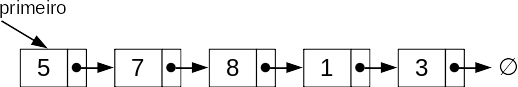
\includegraphics[height=0.15\paperheight]{imagens/lista_simplesmente_encadeada2.png}
\end{figure}
	\item Ao inserir um elemento, deve-se alocar um nodo, preenchê-lo e colocá-lo na posição desejada na estrutura (ajustando as referências necessárias)
	\item Ao remover um elemento, é preciso removê-lo (ajustando as referências necessárias) e desalocá-lo
\end{itemize}
\end{frame}

%-------------------------------------------------------
\begin{frame}[fragile]\frametitle{Estruturas Encadeadas em C++}
\begin{itemize}
	\item Pode-se declarar um nodo em C++, para armazenar caracteres, da seguinte forma:
\begin{lstlisting}[basicstyle=\ttfamily\scriptsize]
struct Node {
  char info;
  Node *next;
  Node(char l) {
    info = l;
    next = nullptr;
  }
};
\end{lstlisting}
	\item \texttt{nullptr} é usado para indicar uma estrutura vazia ou fim da estrutura
	\item Exemplo: construção da seguinte pilha simplesmente encadeada
\begin{figure}[h]
	\centering
	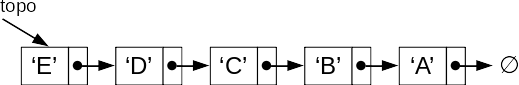
\includegraphics[height=0.15\paperheight]{imagens/pilha_simplesmente_encadeada.png}
\end{figure}
\end{itemize}
\end{frame}

%-------------------------------------------------------
\begin{frame}[fragile]\frametitle{Exemplo: \texttt{pilha\_simplesmente\_encadeada.cpp}}
\fontsize{5pt}{5pt}\selectfont{
\lstinputlisting{src/pilha_simplesmente_encadeada.cpp}
}
\end{frame}

%=======================================================
\section{Exercícios}

%-------------------------------------------------------
\begin{frame}[fragile]\frametitle{Exercícios 6 e 7}
\begin{enumerate}
	\setcounter{enumi}{5}
	\item Modifique o programa da lâmina anterior para que a lista seja criada \textbf{com um laço}, exatamente com o mesmo conteúdo e na mesma ordem lógica. Faça as inserções sempre pela mesma extremidade da estrutura encadeada.
	\item Usando como modelo o programa da lâmina anterior, construa em C++ a seguinte lista duplamente encadeada. Percorra a lista, mostrando o conteúdo de seus nodos, tanto do início para o fim, quanto do fim para o início.
\begin{figure}[h]
	\centering
	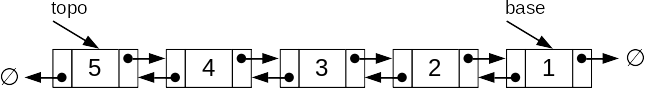
\includegraphics[height=0.16\paperheight]{imagens/pilha_duplamente_encadeada.png}
\end{figure}
\end{enumerate}
\end{frame}

%-------------------------------------------------------
\begin{frame}[fragile]\frametitle{Exercício 8}
\begin{enumerate}
        \setcounter{enumi}{7}
	\item Usando como ponto de partida a classe \texttt{IntStack}, apresentada anteriormente e implementada usando alocação sequencial ou contígua, implemente a classe \texttt{IntLinkedStack}, que funciona da mesma forma, porém usando alocação encadeada.\\
	Observações:
	\begin{itemize}
		\item A versão usando alocação encadeada eliminará a necessidade de se trabalhar com um limite máximo de elementos, consequentemente, os métodos \texttt{maxSize()} e \texttt{isFull()} NÃO farão parte da nova implementação.
		\item A definição da classe (arquivo \texttt{IntLinkedStack.hpp}) e um programa de teste (arquivo \texttt{IntLinkedStackMain.cpp}) estão listados nas lâminas a seguir.
	\end{itemize}
\end{enumerate}
\end{frame}

%-------------------------------------------------------
\begin{frame}[fragile]\frametitle{Exercício 8: \texttt{IntLinkedStack.hpp}}
\lstinputlisting[basicstyle=\ttfamily\tiny]{src/IntLinkedStack.hpp}
\end{frame}

%-------------------------------------------------------
\begin{frame}[fragile]\frametitle{Exercício 8: \texttt{IntLinkedStackMain.cpp}}
\fontsize{6pt}{6pt}\selectfont{
\lstinputlisting{src/IntLinkedStackMain.cpp}
}
\end{frame}

%=======================================================
\section{Fila (\emph{Queue})}

%-------------------------------------------------------
\begin{frame}\frametitle{Fila ou \emph{Queue}}
\begin{itemize}
	\item Usa a política \emph{FIFO -- First In First Out} (o primeiro que entrou, é o primeiro a sair)
	\item Possui uma entrada (fim), a partir da qual os dados são inseridos, e uma saída (início), a partir da qual os dados são removidos
\begin{figure}[h]
	\centering
	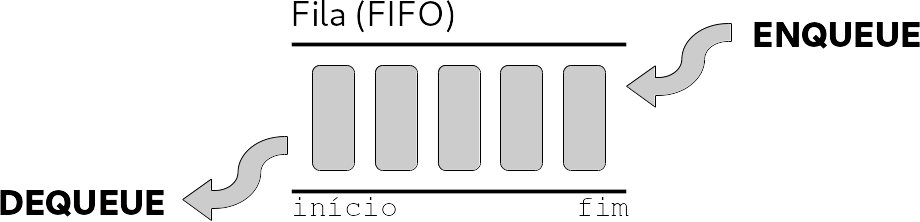
\includegraphics[height=0.3\paperheight]{imagens/fila.png}
\end{figure}
\end{itemize}
\end{frame}

%-------------------------------------------------------
\begin{frame}\frametitle{Aplicações que Usam Fila}
\begin{itemize}
	\item Desenvolvimento de aplicativos
	\begin{itemize}
		\item Gerenciamento de transações para aplicativos de lojas, teatros, centros de reserva, etc.
	\end{itemize}
	\item Simulações
	\begin{itemize}
		\item Listas de espera na simulação de sistemas de atendimento (banco, supermercado, etc.)
	\end{itemize}
	\item Sistemas Operacionais
	\begin{itemize}
		\item Fila de documentos para impressão
		\item Escalonamento de processos em um sistema operacional
		\item Fila de requisições de acesso a disco
		\item Fila de espera por recursos
		\item Fila (\emph{buffering}) de mensagens e pacotes
	\end{itemize}
	\item Estruturas de Dados
	\begin{itemize}
		\item Suporte na implementação de algoritmos sobre árvores e grafos
	\end{itemize}
	\item etc.
\end{itemize}
\end{frame}

%-------------------------------------------------------
\begin{frame}\frametitle{Fila: Implementações Possíveis}
\begin{itemize}
	\item \textbf{Arranjo (\emph{buffer}) circular}
\begin{figure}[h]
	\flushleft
	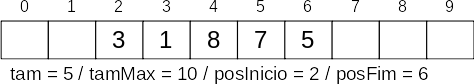
\includegraphics[height=0.13\paperheight]{imagens/fila1a.png} ~ ~ ~ 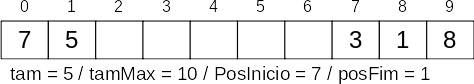
\includegraphics[height=0.13\paperheight]{imagens/fila1b.png}
\end{figure}
	\item \textbf{Lista Simplesmente Encadeada}
\begin{figure}[h]
	\flushleft
	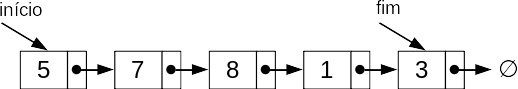
\includegraphics[height=0.15\paperheight]{imagens/fila2.png}
\end{figure}
	\item \textbf{Lista Duplamente Encadeada}
\begin{figure}[h]
	\flushleft
	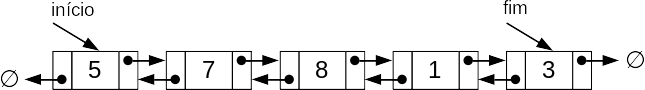
\includegraphics[height=0.15\paperheight]{imagens/fila3.png}
\end{figure}
\end{itemize}
\end{frame}

%-------------------------------------------------------
\begin{frame}[fragile]\frametitle{Implementação de um Arranjo Circular}
\begin{itemize}
	\item Usam-se índices para inserção (\texttt{insertPos}) e remoção (\texttt{removePos}) que percorrem o arranjo (\texttt{queue}) de forma ``circular''
	\item Para inserir pode-se usar:
\begin{lstlisting}[basicstyle=\ttfamily\scriptsize]
queue[ insertPos++ ] = e;
insertPos %= maxElements; // Ou: if ( insertPos == maxElements ) insertPos = 0;
\end{lstlisting}
	\item Para remover pode-se usar:
\begin{lstlisting}[basicstyle=\ttfamily\scriptsize]
e = queue[ removePos++ ];
removePos %= maxElements; // Ou: if ( removePos == maxElements ) removePos = 0;
\end{lstlisting}
	\item Deve-se verificar as situações de arranjo cheio (na inserção) e arranjo vazio (na remoção)
	\item Exemplos:
\begin{figure}[h]
	\flushleft
	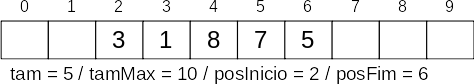
\includegraphics[height=0.13\paperheight]{imagens/fila1a.png} ~ ~ ~ 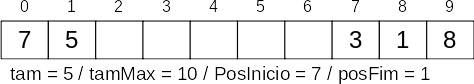
\includegraphics[height=0.13\paperheight]{imagens/fila1b.png}
\end{figure}
\end{itemize}
\end{frame}

%-------------------------------------------------------
\begin{frame}\frametitle{Métodos do TAD Fila (\emph{Queue})}
\begin{itemize}
	\item \texttt{bool enqueue(e)}: insere o elemento no final da fila (retorna \texttt{true}, em caso de sucesso, ou \texttt{false}, se NÃO houver espaço)
	\item \texttt{bool dequeue(\&e)}: remove e retorna (por referência) o elemento do início da fila (retorna \texttt{true}, em caso de sucesso, ou \texttt{false}, a fila estiver vazia)
	\item \texttt{bool head(\&e)} ou \texttt{bool front(\&e)}: retorna (por referência) o elemento do início da fila, mas não o remove da fila (retorna \texttt{true}, em caso de sucesso, ou \texttt{false}, a fila estiver vazia)
	\item \texttt{int size()}: retorna o número de elementos da fila
	\item \texttt{int maxSize()}: retorna o número máximo de elementos suportado pela fila
	\item \texttt{bool isEmpty()}: retorna \texttt{true}, se a fila estiver vazia, ou \texttt{false}, em caso contrário
	\item \texttt{bool isFull()}: retorna \texttt{true}, se a fila estiver cheia, ou \texttt{false}, em caso contrário
	\item \texttt{void clear()}: esvazia a fila
\end{itemize}
\end{frame}

%-------------------------------------------------------
\begin{frame}\frametitle{Exemplo de Implementação: \texttt{IntQueue.hpp}}
\lstinputlisting[basicstyle=\ttfamily\tiny]{src/IntQueue.hpp}
\end{frame}

%-------------------------------------------------------
\begin{frame}\frametitle{Exemplo de Implementação: \texttt{IntQueue.cpp}}
\fontsize{3pt}{5pt}\selectfont{
\lstinputlisting{src/IntQueue.cpp}
}
\end{frame}

%-------------------------------------------------------
\begin{frame}\frametitle{Exemplo de Implementação: \texttt{IntQueueMain.cpp}}
\fontsize{5pt}{6pt}\selectfont{
\lstinputlisting{src/IntQueueMain.cpp}
}
\end{frame}
%-------------------------------------------------------
\begin{frame}\frametitle{Exemplo de Implementação (Saída)}
\lstinputlisting[basicstyle=\ttfamily\scriptsize]{src/IntQueueApp.output}
\end{frame}

%=======================================================
\section{Exercícios}

%-------------------------------------------------------
\begin{frame}[fragile]\frametitle{Exercício 9}
\begin{enumerate}
	\setcounter{enumi}{8}
	\item Considere duas estrutura de dados do tipo fila, chamadas \texttt{A} e \texttt{B}. Na fila \texttt{A}, foram inseridos (nessa ordem) os seguintes valores: 10, 20 e 30. E, na fila \texttt{B}, foram inseridos (nessa ordem) os seguintes valores: 30, 20 e 10. Para ambas as estruturas, considere as seguintes operações:
\begin{itemize}
	\item \texttt{dequeue(F)}: que remove um elemento da fila \texttt{F} e retorna esse elemento;
	\item \texttt{enqueue(F, E)}: que insere o elemento \texttt{E} na fila \texttt{F};
	\item \texttt{head(F)}: que retorna o elemento do início da fila, sem removê-lo da estrutura.
\end{itemize}
Quais serão as sequências de elementos nas filas \texttt{A} e \texttt{B}, após executar a expressão ``\texttt{enqueue(A, dequeue(A) + dequeue(B) + head(A))}''?
\end{enumerate}
\end{frame}

%-------------------------------------------------------
\begin{frame}[fragile]\frametitle{Exercício 10}
\begin{enumerate}
        \setcounter{enumi}{9}
	\item Usando como ponto de partida a classe \texttt{IntQueue}, apresentada anteriormente e implementada usando alocação sequencial ou contígua, implemente a classe \texttt{IntLinkedQueue}, que funciona da mesma forma, porém usando alocação encadeada.\\
	Observações:
	\begin{itemize}
		\item A versão usando alocação encadeada eliminará a necessidade de se trabalhar com um limite máximo de elementos, consequentemente, os métodos \texttt{maxSize()} e \texttt{isFull()} NÃO farão parte da nova implementação.
		\item A definição da classe (arquivo \texttt{IntLinkedQueue.hpp}) e um programa de teste (arquivo \texttt{IntLinkedQueueMain.cpp}) estão listados nas lâminas a seguir.
	\end{itemize}
\end{enumerate}
\end{frame}

%-------------------------------------------------------
\begin{frame}[fragile]\frametitle{Exercício 10: \texttt{IntLinkedQueue.hpp}}
\lstinputlisting[basicstyle=\ttfamily\tiny]{src/IntLinkedQueue.hpp}
\end{frame}

%-------------------------------------------------------
\begin{frame}[fragile]\frametitle{Exercício 10: \texttt{IntLinkedQueueMain.cpp}}
\fontsize{6pt}{6pt}\selectfont{
\lstinputlisting{src/IntLinkedQueueMain.cpp}
}
\end{frame}

%=======================================================
\section{Deque}

%-------------------------------------------------------
\begin{frame}\frametitle{Deque}
\begin{itemize}
	\item É uma abreviação de \emph{Double-Ended QUEue}
	\item Trata-se de uma estrutura linear de dados, um pouco mais flexível do que pilhas ou filas, que permite inserções e remoções tanto no início quanto no final
	\item Possui, portanto, duas pontas (\texttt{frente} e \texttt{traseira} ou \texttt{front} e \texttt{back}), sendo possível selecionar qual será utilizada tanto para inserção quanto para remoção
\begin{figure}[h]
	\centering
	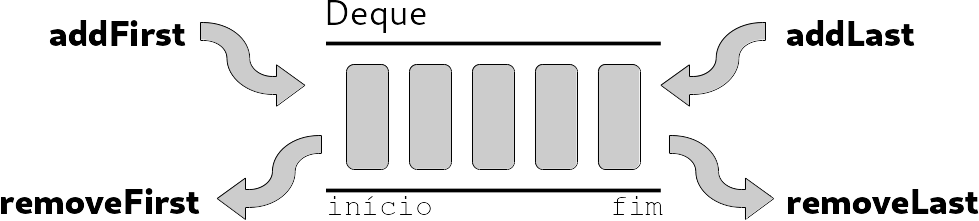
\includegraphics[height=0.3\paperheight]{imagens/deque.png}
\end{figure}
\end{itemize}
\end{frame}

%-------------------------------------------------------
\begin{frame}\frametitle{Deque: Aplicações e Implementações}
\begin{itemize}
	\item É usado em aplicações onde, por exemplo:
	\begin{itemize}
		\item Um item é removido da fila e por alguma razão precisa ser reinserido na posição que ocupava anteriormente
		\item O último item da fila ``desiste'' de permanecer nela (por exemplo, devido à demora ou ao tamanho da fila)
	\end{itemize}
	\item Pode ser implementado da mesma forma que uma fila:
	\begin{itemize}
		\item Arranjo (\emph{buffer}) circular
		\item Lista Simplesmente Encadeada
		\item Lista Duplamente Encadeada
	\end{itemize}
	\item Há implementações bloqueantes, em que a primitiva de inserção fica bloqueada até haver espaço e a primitiva de remoção fica bloqueada até que exista um elemento para ser removido
\end{itemize}
\end{frame}

%-------------------------------------------------------
\begin{frame}\frametitle{Métodos do TAD Deque}
\begin{itemize}
{\scriptsize
	\item \texttt{bool addFirst(e)}: insere o elemento no início do deque (retorna \texttt{true}, em caso de sucesso, ou \texttt{false}, se NÃO houver espaço)\\
	\item \texttt{bool addLast(e)}: insere o elemento no fim do deque (retorna \texttt{true}, em caso de sucesso, ou \texttt{false}, se NÃO houver espaço)\\
	\item \texttt{bool removeFirst(\&e)}: remove e retorna (por referência) o elemento do início do deque (retorna \texttt{true}, em caso de sucesso, ou \texttt{false}, o deque estiver vazio)\\
	\item \texttt{bool removeLast(\&e)}: remove e retorna (por referência) o elemento do fim do deque (retorna \texttt{true}, em caso de sucesso, ou \texttt{false}, o deque estiver vazio)\\
	\item \texttt{bool first(\&e)} ou \texttt{bool head(\&e)} ou \texttt{bool front(\&e)}: retorna (por referência) o elemento do início do deque, mas não o remove do deque (retorna \texttt{true}, em caso de sucesso, ou \texttt{false}, o deque estiver v\\azio)
	\item \texttt{bool last(\&e)} ou \texttt{bool tail(\&e)} ou \texttt{bool back(\&e)}: retorna (por referência) o elemento do fim do deque, mas não o remove do deque (retorna \texttt{true}, em caso de sucesso, ou \texttt{false}, o deque estiver vazio)\\
	\item \texttt{int size()}: retorna o número de elementos do deque\\
	\item \texttt{int maxSize()}: retorna o número máximo de elementos suportado pelo deque\\
	\item \texttt{bool isEmpty()}: retorna \texttt{true}, se o deque estiver vazio, ou \texttt{false}, em caso contrário\\
	\item \texttt{bool isFull()}: retorna \texttt{true}, se o deque estiver cheio, ou \texttt{false}, em caso contrário\\
	\item \texttt{void clear()}: esvazia o deque\\
}
\end{itemize}
\end{frame}

%=======================================================
\section{Exercícios}

%-------------------------------------------------------
\begin{frame}[fragile]\frametitle{Exercício 11}
\begin{enumerate}
        \setcounter{enumi}{10}
{\footnotesize
	\item Considere as seguintes declarações para uma estrutura linear duplamente encadeada do tipo deque:
\begin{lstlisting}[basicstyle=\ttfamily\tiny]
  struct Node {
    char info;  Node *prev, *next;
    Node(char i) {  info = i;  prev = next = nullptr;  }
  };
  Node *esquerda = nullptr, *direita = nullptr;
\end{lstlisting}
E determine o estado final, na ordem correta, dos ponteiros e dos nodos dessa estrutura, depois da execução das seguintes operaçõess:
	\begin{itemize}
{\scriptsize
		\item Inserir as letras 'D', 'E', 'S', 'C', 'A', 'R', 'T', 'E' e 'S' (nesta ordem), cada uma em um nodo da lista, pela direita;
		\item Remover 3 letras do deque pela esquerda;
		\item Remover 4 letras do deque pela direita;
		\item Inserir as letras 'E', 'D', 'I', 'S', 'O' e 'N' (nesta ordem), cada uma em um nodo da lista, pela esquerda;
		\item Remover 5 letras do deque pela esquerda;
		\item Inserir as letras 'R', 'U', 'T', 'H', 'E', 'R', 'F', 'O', 'R' e 'D' (nesta ordem), cada uma em um nodo da lista, pela esquerda;
		\item Remover 8 letras do deque pela esquerda;
		\item Inserir as letras 'E', 'I', 'N', 'S', 'T', 'E', 'I' e 'N' (nesta ordem), cada uma em um nodo da lista, pela esquerda;
		\item Remover 7 letras do deque pela esquerda.
}
	\end{itemize}
}
\end{enumerate}
\end{frame}

%-------------------------------------------------------
\begin{frame}[fragile]\frametitle{Exercício 12}
\begin{enumerate}
        \setcounter{enumi}{11}
	\item Usando como ponto de partida os códigos apresentados e desenvolvidos anteriormente, implemente a classe \texttt{IntDoubleLinkedDeque}, que implementa um deque com uma lista duplamente encadeada.\\
	Observações:
	\begin{itemize}
		\item Lembre-se que NÃO haverá necessidade de trabalhar com um limite máximo de elementos, consequentemente, os métodos \texttt{maxSize()} e \texttt{isFull()} NÃO farão parte da nova implementação.
		\item A definição da classe (arquivo \texttt{IntDoubleLinkedDeque.hpp}) e um programa de teste (arquivo \texttt{IntDoubleLinkedDequeMain.cpp}) estão listados nas lâminas a seguir.
	\end{itemize}
\end{enumerate}
\end{frame}

%-------------------------------------------------------
\begin{frame}[fragile]\frametitle{Exercício 12: \texttt{IntDoubleLinkedDeque.hpp}}
\lstinputlisting[basicstyle=\ttfamily\tiny]{src/IntDoubleLinkedDeque.hpp}
\end{frame}

%-------------------------------------------------------
\begin{frame}[fragile]\frametitle{Exercício 12: \texttt{IntDoubleLinkedDequeMain.cpp}}
\fontsize{6pt}{6pt}\selectfont{
\lstinputlisting{src/IntDoubleLinkedDequeMain.cpp}
}
\end{frame}

%=======================================================
\section{Lista}

%-------------------------------------------------------
\begin{frame}\frametitle{Lista}
\begin{itemize}
	\item Uma lista é uma estrutura de dados que agrupa informações referentes a um conjunto de elementos relacionados entre si
	\item Há uma ordem lógica entre os elementos, que não corresponde necessariamente à ordem física
	\item A inserção e exclusão em uma lista é menos restritiva do que em pilhas, filas ou deques
	\item Isto significa que uma implementação de lista poderia ser usada para criar e gerenciar pilhas, filas e deques
\end{itemize}
\end{frame}

%-------------------------------------------------------
\begin{frame}\frametitle{Operações sobre Listas}
\begin{itemize}
	\item Algumas operações básicas sobre listas, envolvendo elementos (nodos), são:
	\begin{itemize}
		\item Inserção (no início, no fim ou em uma posição específica)
		\item Remoção (no início, no fim ou em uma posição específica)
		\item Busca e acesso (através de índice ou através da informação de algum campo)
		\item Alteração
	\end{itemize}
	\item Também é comum aplicar operações sobre toda a lista, tais como:
	\begin{itemize}
		\item Combinação de duas ou mais listas em uma única lista (concatenação ou \emph{merge})
		\item Ordenação da lista segundo determinado critério
	\end{itemize}
\end{itemize}
\end{frame}

%-------------------------------------------------------
\begin{frame}\frametitle{Opções de Implementação}
\begin{itemize}
	\item Usando arranjos
	\begin{itemize}
		\item Maior desempenho no acesso
		\item Apresentam maior dificuldade de inserção e remoção no início ou no meio
	\end{itemize}
	\item Usando estruturas encadeadas
	\begin{itemize}
		\item Menor desempenho no acesso
		\item Muito mais flexível para inserir e remover nodos
		\item Podem ser: simplesmente encadeadas, duplamente encadeadas, simplesmente encadeadas e circulares, duplamente encadeadas e circulares
	\end{itemize}
\end{itemize}
\end{frame}

%=======================================================
\section{Lista com Arranjo}

%-------------------------------------------------------
\begin{frame}\frametitle{Lista com Arranjo}
\begin{itemize}
	\item Consiste em um número fixo de posições \textbf{contíguas} e para o armazenamento de elementos do mesmo tipo
	\item Possui acesso direto facilitado e rápido, ou seja, o tempo de acesso é constante para qualquer elemento
	\item A inserção e a remoção de nodos no início ou no meio do arranjo tem alto custo, pois requer a movimentação de nodos ou para abrir espaço ou para evitar espaços não utilizados
	\item Geralmente é preciso definir o número máximo de elementos que serão armazenados (mudar esse tamanho pode ser possível, mas será custoso)
\begin{figure}[h]
	\centering
	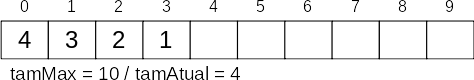
\includegraphics[height=0.15\paperheight]{imagens/lista_com_arranjo.png}
\end{figure}
\end{itemize}
\end{frame}

%-------------------------------------------------------
\begin{frame}\frametitle{Métodos para um TAD Lista com Arranjo}
\begin{itemize}
{\scriptsize
	\item \texttt{bool add(e)}: insere o elemento no final da lista (retorna \texttt{true}, em caso de sucesso, ou \texttt{false}, se NÃO houver espaço)
	\item \texttt{bool add(index,e)}: insere o elemento em um índice específico da lista (retorna \texttt{true}, em caso de sucesso, ou \texttt{false}, se NÃO houver espaço)
	\item \texttt{bool get(index, \&e)}: retorna (por referência) o elemento do índice especificado (retorna \texttt{true}, em caso de sucesso, ou \texttt{false}, se o índice for inválido)
	\item \texttt{bool set(index, e)}: atribui o elemento para a posição do índice especificado (retorna \texttt{true}, em caso de sucesso, ou \texttt{false}, se o índice for inválido)
	\item \texttt{bool remove(index)}: remove o elemento do índice especificado da lista (retorna \texttt{true}, em caso de sucesso, ou \texttt{false}, se o índice for inválido)
	\item \texttt{int size()}: retorna o número de elementos da lista\\
	\item \texttt{int maxSize()}: retorna o número máximo de elementos suportado pela lista\\
	\item \texttt{bool isEmpty()}: retorna \texttt{true}, se a lista estiver vazia, ou \texttt{false}, em caso contrário\\
	\item \texttt{bool isFull()}: retorna \texttt{true}, se a lista estiver cheia, ou \texttt{false}, em caso contrário\\
	\item \texttt{bool contains(e)}: retorna \texttt{true}, se o elemento existir na lista, ou \texttt{false},  em caso contrário\\
	\item \texttt{int indexOf(e)}: retorna o índice da primeira ocorrência do elemento na lista, se o elemento existir na lista, ou -1 em caso contrário\\
	\item \texttt{int indexOf(pos,e)}: retorna o índice da próxima ocorrência do elemento na lista a partir da posição especificada, se o elemento existir, ou -1 em caso contrário\\
	\item \texttt{void clear()}: esvazia a lista\\
}
\end{itemize}
\end{frame}

%-------------------------------------------------------
\begin{frame}\frametitle{Lista com Arranjo: Inserção e Exclusão}
\begin{itemize}
	\item Inserção: \texttt{arrayList->add(3,35)}
\begin{figure}[h]
	\centering
	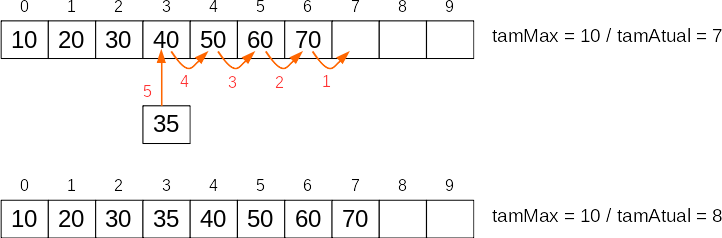
\includegraphics[height=0.30\paperheight]{imagens/lista_com_arranjo_insercao.png}
\end{figure}
	\item Exclusão: \texttt{arrayList->remove(2)}
\begin{figure}[h]
	\centering
	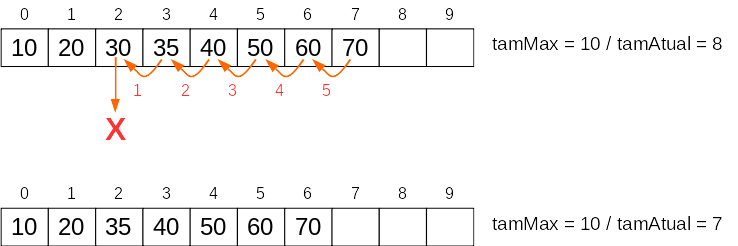
\includegraphics[height=0.30\paperheight]{imagens/lista_com_arranjo_exclusao.png}
\end{figure}
\end{itemize}
\end{frame}

%=======================================================
\section{Exercício}

%-------------------------------------------------------
\begin{frame}[fragile]\frametitle{Exercício 13}
\begin{enumerate}
	\setcounter{enumi}{11}
	\item Usando como base a descrição dos métodos de um TAD Lista com Arranjo, implemente os métodos da classe \texttt{StringArrayList}, que implementa uma lista com um arranjo de tamanho predefinido. O arquivo de cabeçalho para esta classe (\texttt{StringArrayList.hpp}) e um programa de teste (\texttt{StringArrayListMain.cpp}).
\end{enumerate}
\end{frame}

%-------------------------------------------------------
\begin{frame}[fragile]\frametitle{Exercício 13: \texttt{StringArrayList.hpp}}
\fontsize{6pt}{6pt}\selectfont{
\lstinputlisting{src/StringArrayList.hpp}
}
\end{frame}

%-------------------------------------------------------
\begin{frame}[fragile]\frametitle{Exercício 13: \texttt{StringArrayListMain.cpp}}
\fontsize{3pt}{5pt}\selectfont{
\lstinputlisting{src/StringArrayListMain.cpp}
}
\end{frame}

%=======================================================
\section{Lista Encadeada}

%-------------------------------------------------------
\begin{frame}\frametitle{Lista Encadeada}
\begin{itemize}
	\item Armazena elementos do mesmo tipo em uma estrutura formada por nodos (não necessariamente contíguos na memória), cada nodo contendo uma referência para o nodo seguinte (lista simplesmente encadeada) e eventualmente também uma referência para o nodo anterior (lista duplamente encadeada)
\begin{figure}[h]
	\centering
	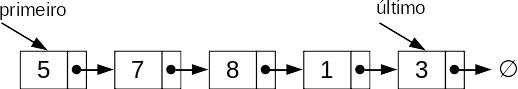
\includegraphics[height=0.12\paperheight]{imagens/lista_simplesmente_encadeada.png} ~ 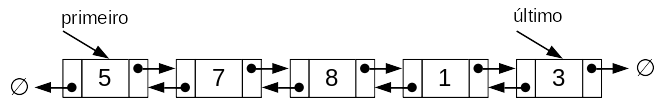
\includegraphics[height=0.12\paperheight]{imagens/lista_duplamente_encadeada.png}
\end{figure}
	\item Para acessar determinado elemento, será preciso percorrer a lista...
	\item No entanto, inserir elementos na lista ou removê-los não exigirá deslocamentos de nodos, apenas ajustes em algumas poucas referências!
\end{itemize}
\end{frame}

%-------------------------------------------------------
\begin{frame}\frametitle{Métodos para um TAD Lista Encadeada}
\begin{itemize}
{\scriptsize
	\item \texttt{int size()}: retorna o número de elementos da lista\\
	\item \texttt{bool isEmpty()}: retorna \texttt{true}, se a lista estiver vazia, ou \texttt{false}, em caso contrário\\
	\item \texttt{void clear()}: esvazia a lista\\
	\item \texttt{void push\_front(e)}: insere o elemento no início da lista\\
	\item \texttt{void push\_back(e)}: insere o elemento no final da lista\\
	\item \texttt{bool insert(index, e)}: insere o elemento no índice especificado da lista\\
	\item \texttt{bool pop\_front()}: remove o elemento do início da lista (retorna \texttt{false} se a lista estiver vazia)\\
	\item \texttt{bool pop\_back()}: remove o elemento do final da lista (retorna \texttt{false} se a lista estiver vazia)\\
	\item \texttt{bool remove(index)}: remove o elemento do índice especificado da lista (retorna \texttt{true}, em caso de sucesso, ou \texttt{false}, se o índice for inválido)\\
	\item \texttt{bool get(index, \&e)}: retorna (por referência) o elemento do índice especificado (retorna \texttt{true}, em caso de sucesso, ou \texttt{false}, se o índice for inválido)\\
	\item \texttt{bool set(index, e)}: atribui o elemento para a posição do índice especificado (retorna \texttt{true}, em caso de sucesso, ou \texttt{false}, se o índice for inválido)\\
	\item \texttt{bool contains(e)}: retorna \texttt{true}, se o elemento existir na lista, ou \texttt{false}, em caso contrário\\
	\item \texttt{int indexOf(e)}: retorna o índice da primeira ocorrência do elemento na lista, ou -1 se o elemento não existir\\
	\item \texttt{int indexOf(pos,e)}: retorna o índice da próxima ocorrência do elemento na lista a partir da posição especificada, ou -1 se o elemento não existir a partir dessa posição\\
}	
\end{itemize}
\end{frame}

%=======================================================
\section{Lista Simplesmente Encadeada}

%-------------------------------------------------------
\begin{frame}[fragile]\frametitle{Lista Simplesmente Encadeada}
\begin{itemize}
	\item É uma estrutura encadeada onde cada nodo, além da informação, guarda apenas uma referência para o próximo nodo
\begin{figure}[h]
	\centering
	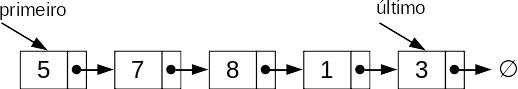
\includegraphics[height=0.15\paperheight]{imagens/lista_simplesmente_encadeada.png}
\end{figure}
	\item Em C++, usando \texttt{struct}, seria possível declarar, por exemplo, uma lista simplesmente encadeada de valores inteiros usando:
\begin{lstlisting}[basicstyle=\ttfamily\scriptsize]
struct Node {
  int info;
  Node *next;
  Node(int i) {  info = i;  next = nullptr;  }
};
\end{lstlisting}
	\item Pode-se trabalhar com dois ponteiros, um para o início (por exemplo, \texttt{head}) e outro (opcional, mas desejável) para o fim da lista (por exemplo, \texttt{tail})
\begin{lstlisting}[basicstyle=\ttfamily\scriptsize]
Node *head = nullptr, *tail = nullptr;
\end{lstlisting}
\end{itemize}
\end{frame}

%-------------------------------------------------------
\begin{frame}[fragile]\frametitle{Lista Simplesmente Encadeada}
\begin{itemize}
	\item Inserir ou remover em uma lista simplesmente encadeada exige localizar o elemento anterior, o que pode exigir percorrer a lista a partir do início
	\begin{itemize}
		\item Inserir ou remover no meio de uma lista duplamente encadeada é mais simples
	\end{itemize}
	\item Para inserir em uma lista encadeada é preciso: alocar um novo nodo, inserir as informações nele e encadeá-lo na lista
	\item Para remover de uma lista encadeada é preciso: recuperar a informação (se necessário), ajustar os encadeamentos da lista e desalocar o nodo
	\item Operações em listas simplesmente encadeadas
	\begin{itemize}
		\item Inserção no início: simples
		\item Inserção no meio: exige referência para o elemento anterior
		\item Inserção no final: simples
		\item Remoção do início: simples
		\item Remoção do meio: exige referência para o elemento anterior
		\item Remoção do final: exige referência para o elemento anterior
	\end{itemize}
\end{itemize}
\end{frame}

%-------------------------------------------------------
\begin{frame}[fragile]\frametitle{Lista Simplesmente Encadeada: Inserção}
\begin{itemize}
	\item Inserção no início
\begin{lstlisting}[basicstyle=\ttfamily\scriptsize]
Node *node = new Node(info);
node->next = head;
head = node;
if ( tail == nullptr ) tail = node;
\end{lstlisting}
	\item Inserção no meio
\begin{lstlisting}[basicstyle=\ttfamily\scriptsize]
// aux aponta para nodo antes do qual se quer inserir
// ant aponta para nodo anterior a aux
Node *node = new Node(info);
ant->next = node;
node->next = aux;
\end{lstlisting}
	\item Inserção no final
\begin{lstlisting}[basicstyle=\ttfamily\scriptsize]
Node *node = new Node(info);
tail->next = node;
tail = node;
\end{lstlisting}
\end{itemize}
\end{frame}

%-------------------------------------------------------
\begin{frame}[fragile]\frametitle{Lista Simplesmente Encadeada: Remoção}
\begin{itemize}
	\item Remoção do início
\begin{lstlisting}[basicstyle=\ttfamily\tiny]
if ( head != nullptr ) {
   Node *aux = head;
   head = head->next;
   if ( head == nullptr ) tail = nullptr;
   delete aux;
}
\end{lstlisting}
	\item Remoção do meio
\begin{lstlisting}[basicstyle=\ttfamily\tiny]
// aux aponta para nodo que se quer remover
// ant aponta para nodo anterior a aux
ant->next = aux->next;
if ( aux->next == nullptr ) tail = ant;
delete aux;
\end{lstlisting}
	\item Remoção do final
\begin{lstlisting}[basicstyle=\ttfamily\tiny]
// ant aponta para nodo anterior a tail
ant->next = nullptr;
delete tail;
tail = ant;
\end{lstlisting}
\end{itemize}
\end{frame}

%=======================================================
\section{Exercícios}

%-------------------------------------------------------
\begin{frame}[fragile]\frametitle{Exercício 14}
\begin{enumerate}
{\footnotesize
	\setcounter{enumi}{13}
	\item Considere o código abaixo, que cria uma lista simplesmente encadeada formada por 4 nodos, respectivamente, com as letras 'B', 'C', 'E' e 'F' como conteúdo. Modifique este código para inserir na lista, \textbf{no ponto indicado no código}, um nodo com a letra 'D', na posição correta da lista, mantendo-se a ordem alfabética crescente. Depois, teste o seu código (e adapte-o se necessário) para inserir, na posição correta, tanto a letra 'A' quanto a letra 'G'.\\

\fontsize{5pt}{5pt}\selectfont{
\lstinputlisting{src/exercicio14.cpp}
}
}
\end{enumerate}
\end{frame}

%-------------------------------------------------------
\begin{frame}[fragile]\frametitle{Exercício 15}
\begin{enumerate}
{\footnotesize
	\setcounter{enumi}{14}
	\item Considere o código abaixo, que cria uma lista simplesmente encadeada formada por 5 nodos, respectivamente, com as letras 'A', 'D', 'C', 'B' e 'E' como conteúdo. Modifique este código para trocar, \textbf{no ponto indicado no código}, a posição dos nodos que contêm 'D' e 'B' na lista.\\
\fontsize{6pt}{6pt}\selectfont{
\lstinputlisting{src/exercicio15.cpp}
}
}
\end{enumerate}
\end{frame}

%-------------------------------------------------------
\begin{frame}[fragile]\frametitle{Exercício 16}
\begin{enumerate}
{\small
	\setcounter{enumi}{15}
	\item Implemente uma aplicação para gerenciar uma \textbf{lista simplesmente encadeada} em que os nós armazenam uma letra (\texttt{char}) e um ponteiro para o próximo elemento. A aplicação deve permitir interativamente a inserção de letras na lista a partir de um pequeno conjunto de operações fornecidas pela entrada padrão (terminal). As operações e seus parâmetros são indicadas pelos seguintes caracteres:
	\begin{itemize}
	{\scriptsize
		\item '<' (menor) e letra: insere a letra especificada no início da lista;
		\item '>' (maior) e letra: insere a letra especificada no fim da lista;
		\item '+' (mais), letra e índice: insere a letra especificada no índice especificado da lista;
		\item '\{' (abre-chaves): remove a letra/nodo do início da lista (imprime ``ERRO'' se a lista estiver vazia);
		\item '\}' (fecha-chaves): remove a letra/nodo do final da lista (imprime ``ERRO'' se a lista estiver vazia);
		\item '-' (menos) e índice: remove o elemento no índice especificado (imprime ``ERRO'' se o índice for inválido);
		\item '.' (ponto): encerra a aplicação.
	}
	\end{itemize}
	No laço principal da sua aplicação, sempre antes de ler a especificação de uma operação, mostre o conteúdo da lista. Use o arquivo \texttt{exercicio16.input} (dentro do arquivo \texttt{src.zip}) como entrada para testar o seu programa.
}
\end{enumerate}
\end{frame}

%-------------------------------------------------------
\begin{frame}[fragile]\frametitle{Exercício 16: \texttt{exercicio16-template.cpp}}
\fontsize{5pt}{5pt}\selectfont{
\lstinputlisting{src/exercicio16-template.cpp}
}
\end{frame}

%=======================================================
\section{Lista Duplamente Encadeada}

%-------------------------------------------------------
\begin{frame}[fragile]\frametitle{Lista Duplamente Encadeada}
\begin{itemize}
	\item É uma estrutura encadeada onde cada nodo, além da informação, guarda uma referência para o próximo nodo e uma referência para o nodo anterior
\begin{figure}[h]
	\centering
	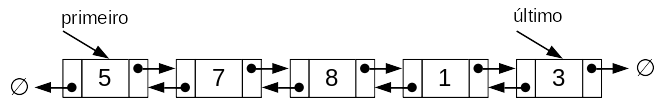
\includegraphics[height=0.15\paperheight]{imagens/lista_duplamente_encadeada.png}
\end{figure}
	\item Em C++, usando \texttt{struct}, seria possível declarar, por exemplo, uma lista simplesmente encadeada de valores inteiros usando:
\begin{lstlisting}[basicstyle=\ttfamily\scriptsize]
struct Node {
  int info;
  Node *prev, *next;
  Node(int i) {  info = i;  prev = next = nullptr;  }
};
\end{lstlisting}
	\item Também são usados dois ponteiros, um para o início (por exemplo, \texttt{head}) e outro (opcional, mas desejável)	 para o fim da lista (por exemplo, \texttt{tail})
\begin{lstlisting}[basicstyle=\ttfamily\scriptsize]
Node *head = nullptr, *tail = nullptr;
\end{lstlisting}
\end{itemize}
\end{frame}

%-------------------------------------------------------
\begin{frame}[fragile]\frametitle{Lista Duplamente Encadeada}
\begin{itemize}
	\item Para inserir ou remover em uma lista duplamente encadeada basta ter a posição de inserção ou remoção, NÃO sendo necessário percorrer a lista a partir do início
	\begin{itemize}
		\item É mais fácicl inserir ou remover em uma lista duplamente encadeada do que em uma lista simplesmente encadeada
	\end{itemize}
	\item Para inserir em uma lista encadeada é preciso: alocar um novo nodo, inserir as informações nele e encadeá-lo na lista
	\item Para remover de uma lista encadeada é preciso: recuperar a informação (se necessário), ajustar os encadeamentos da lista e desalocar o nodo
\end{itemize}
\end{frame}

%-------------------------------------------------------
\begin{frame}[fragile]\frametitle{Lista Duplamente Encadeada: Inserção}
\begin{itemize}
	\item Inserção no início
\begin{lstlisting}[basicstyle=\ttfamily\tiny]
Node *node = new Node(info);
if ( head == nullptr ) { head = tail = node; }
else {
  node->next = head;
  head->prev = node;
  head = node;
}
\end{lstlisting}
	\item Inserção no meio
\begin{lstlisting}[basicstyle=\ttfamily\tiny]
// aux aponta para nodo antes do qual se quer inserir
Node *node = new Node(info);
node->prev = aux->prev;
node->next = aux;
(aux->prev)->next = node;
aux->prev = node;
\end{lstlisting}
	\item Inserção no final
\begin{lstlisting}[basicstyle=\ttfamily\tiny]
Node *node = new Node(info);
node->prev = tail;
tail->next = node;
tail = node;
\end{lstlisting}
\end{itemize}
\end{frame}

%-------------------------------------------------------
\begin{frame}[fragile]\frametitle{Lista Duplamente Encadeada: Remoção}
\begin{itemize}
	\item Remoção do início
\begin{lstlisting}[basicstyle=\ttfamily\tiny]
if ( head != nullptr ) {
   Node *aux = head;
   head = head->next;
   if ( head == nullptr ) tail = nullptr;
   else head->prev = nullptr;
   delete aux;
}
\end{lstlisting}
	\item Remoção do meio
\begin{lstlisting}[basicstyle=\ttfamily\tiny]
// aux aponta para nodo que se quer remover
(aux->prev)->next = aux->next;
if ( aux->next == nullptr ) tail = aux->prev;
else (aux->next)->prev = aux->prev;
delete aux;
\end{lstlisting}
	\item Remoção do final
\begin{lstlisting}[basicstyle=\ttfamily\tiny]
Node *aux = tail;
tail = tail->prev;
if ( tail == nullptr )  head = nullptr;
else tail->next = nullptr;
delete aux;
\end{lstlisting}
\end{itemize}
\end{frame}

%=======================================================
\section{Exercícios}

%-------------------------------------------------------
\begin{frame}[fragile]\frametitle{Exercício 17}
\begin{enumerate}
{\scriptsize
        \setcounter{enumi}{16}
	\item Considere uma \textbf{lista simplesmente encadeada}, com referências para o início e para o final, cujos nodos foram declarados da seguinte forma:
\begin{lstlisting}[basicstyle=\ttfamily\tiny]
struct Node {
  int info;  Node *next;
  Node(int i) {  info = i;  next = nullptr;  }
};
\end{lstlisting}
Implemente uma função que recebe os ponteiros para o início e para o final da lista (por referência) e inverte a lista. A função deve ter o seguinte protótipo:
\begin{lstlisting}[basicstyle=\ttfamily\tiny]
void reverse(Node **head, Node **tail);
\end{lstlisting}
	\item Considere uma \textbf{lista duplamente encadeada}, com referências para o início e para o final, cujos nodos foram declarados da seguinte forma:
\begin{lstlisting}[basicstyle=\ttfamily\tiny]
struct Node {
  int info;  Node *prev, *next;
  Node(int i) {  info = i;  prev = next = nullptr;  }
};
\end{lstlisting}
Implemente uma função que recebe os ponteiros para o início e para o final da lista (por referência) e inverte a lista. A função deve ter o seguinte protótipo:
\begin{lstlisting}[basicstyle=\ttfamily\tiny]
void reverse(Node **head, Node **tail);
\end{lstlisting}
}
\end{enumerate}
\end{frame}

%=======================================================
\section{Lista Circular}

%-------------------------------------------------------
\begin{frame}[fragile]\frametitle{Lista Circular}
\begin{itemize}
	\item Uma lista circular é um tipo especial de estrutura encadeada onde o último elemento aponta para o primeiro (não usando-se, neste caso, \texttt{nullptr} para indicar o final da lista)
	\item É possível ter listas circulares:
	\begin{itemize}
		\item Simplesmente encadeadas: a busca somente ocorre em um sentido
\begin{lstlisting}[basicstyle=\ttfamily\tiny]
struct Node {
  int info;  Node *next;
  Node(int i) {  info = i;  next = nullptr;  }
};
\end{lstlisting}
		\item Duplamente encadeadas: a busca pode ocorrer em qualquer sentido
\begin{figure}[h]
	\centering
	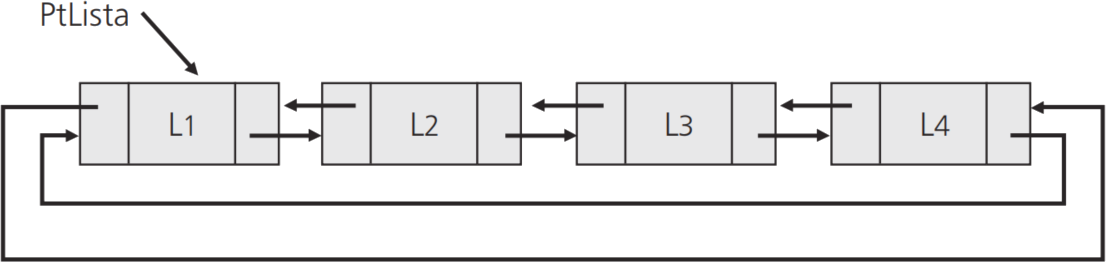
\includegraphics[height=0.14\paperheight]{imagens/lista_circular_duplamente_encadeada.png}
\end{figure}
\begin{lstlisting}[basicstyle=\ttfamily\tiny]
struct Node {
  int info;  Node *prev, *next;
  Node(int i) {  info = i;  prev = next = nullptr;  }
};
\end{lstlisting}
	\end{itemize}
\end{itemize}
\end{frame}

%-------------------------------------------------------
\begin{frame}[fragile]\frametitle{Lista Circular}
\begin{itemize}
	\item Observe que nada muda nas declarações em relação às versões não circulares
	\item Se a lista circular é duplamente encadeada, NÃO há a necessidade de um ponteiro para o final da listas
	\item Com listas circulares simplesmente encadeadas, um ponteiro para o final da lista é desejável
	\item Exemplo de aplicação: \textbf{Lista de processos prontos para serem executados em um sistema operacional com algoritmo de escalonamento \emph{Round Robin}}
	\begin{itemize}
		\item \emph{Round Robin} é um escalonamento preemptivo que divide uniformemente o tempo da UCP entre todos os processos prontos para a execução
		\item Processos são mantidos em uma lista de prontos circular e duplamente encadeada
		\item Cada processo tem uma fatia de tempo máxima (\emph{time slice} ou \emph{quantum}) para usar o processador
		\item Se o processo termina a sua computação antes do final da fatia de tempo, ele sai da lista
		\item Se o processo usa toda a sua fatia de tempo, o ponteiro da lista é apontado para o próximo processo
	\end{itemize}
\end{itemize}
\end{frame}

%=======================================================
\section{Créditos}

%-------------------------------------------------------
\begin{frame}\frametitle{Créditos}
\begin{itemize}
	\item Estas lâminas contêm trechos inspirados em materiais criados e disponibilizados pelos professores Isabel Harb Manssour e Iaçanã Ianiski Weber.
\end{itemize}
\end{frame}

%=======================================================
\section{Soluções}

%-------------------------------------------------------
\begin{frame}[fragile]\frametitle{Exercício 1: \texttt{CharStack.hpp}}
\lstinputlisting[basicstyle=\ttfamily\tiny]{src/CharStack.hpp}
\end{frame}

%-------------------------------------------------------
\begin{frame}[fragile]\frametitle{Exercício 1: \texttt{CharStack.cpp}}
\fontsize{5pt}{5pt}\selectfont{
\lstinputlisting{src/CharStack.cpp}
}
\end{frame}

%-------------------------------------------------------
\begin{frame}[fragile]\frametitle{Exercício 2: \texttt{exercicio02.cpp}}
\lstinputlisting[basicstyle=\ttfamily\tiny]{src/exercicio02.cpp}
\end{frame}

%-------------------------------------------------------
\begin{frame}[fragile]\frametitle{Exercício 3: \texttt{exercicio03.cpp}}
\lstinputlisting[basicstyle=\ttfamily\tiny]{src/exercicio03.cpp}
\end{frame}

%-------------------------------------------------------
\begin{frame}[fragile]\frametitle{Exercício 4: \texttt{exercicio04.cpp}}
\fontsize{5pt}{5pt}\selectfont{
\lstinputlisting{src/exercicio04.cpp}
}
\end{frame}

%-------------------------------------------------------
\begin{frame}[fragile]\frametitle{Exercício 5: \texttt{exercicio05.cpp}}
\lstinputlisting[basicstyle=\ttfamily\tiny]{src/exercicio05.cpp}
\end{frame}

%-------------------------------------------------------
\begin{frame}[fragile]\frametitle{Exercício 6: \texttt{pilha\_simplesmente\_encadeada2.cpp}}
\fontsize{6pt}{6pt}\selectfont{
\lstinputlisting{src/pilha_simplesmente_encadeada2.cpp}
}
\end{frame}

%-------------------------------------------------------
\begin{frame}[fragile]\frametitle{Exercício 7: \texttt{pilha\_duplamente\_encadeada.cpp}}
\fontsize{5pt}{5pt}\selectfont{
\lstinputlisting{src/pilha_duplamente_encadeada.cpp}
}
\end{frame}

%-------------------------------------------------------
\begin{frame}[fragile]\frametitle{Exercício 8: \texttt{IntLinkedStack.cpp}}
\fontsize{3pt}{5pt}\selectfont{
\lstinputlisting{src/IntLinkedStack.cpp}
}
\end{frame}

%-------------------------------------------------------
\begin{frame}[fragile]\frametitle{Exercício 9}
\small{
\begin{verbatim}
// inicial
A = { 10, 20, 30 }   B = { 30, 20, 10 }

// após dequeue(A) tem-se "10 + dequeue(B) + head(A)"
A = { 20, 30 }       B = { 30, 20, 10 }

// após dequeue(B) tem-se "10 + 30 + head(A)"
A = { 20, 30 }       B = { 20, 10 }

// após head(A) tem-se "10 + 30 + 20 = 60"
A = { 20, 30 }       B = { 20, 10 }

// resposta final, após "enqueue(A, 60)"
A = { 20, 30, 60 }   B = { 20, 10 }
\end{verbatim}
}
\end{frame}

%-------------------------------------------------------
\begin{frame}[fragile]\frametitle{Exercício 10: \texttt{IntLinkedQueue.cpp}}
\fontsize{3pt}{5pt}\selectfont{
\lstinputlisting{src/IntLinkedQueue.cpp}
}
\end{frame}

%-------------------------------------------------------
\begin{frame}[fragile]\frametitle{Exercício 11}
\small{
\begin{verbatim}
esquerda --> || <-- direita

esquerda --> |'D'|'E'|'S'|'C'|'A'|'R'|'T'|'E'|'S'| <-- direita
esquerda --> |'C'|'A'|'R'|'T'|'E'|'S'| <-- direita
esquerda --> |'C'|'A'| <-- direita
esquerda --> |'N'|'O'|'S'|'I'|'D'|'E'|'C'|'A'| <-- direita
esquerda --> |'E'|'C'|'A'| <-- direita
esquerda --> |'D'|'R'|'O'|'F'|'R'|'E'|'H'|'T'|'U'|'R'|'E'|'C'|'A'| <-- direita
esquerda --> |'U'|'R'|'E'|'C'|'A'| <-- direita
esquerda --> |'N'|'I'|'E'|'T'|'S'|'N'|'I'|'E'|'U'|'R'|'E'|'C'|'A'| <-- direita

esquerda --> |'E'|'U'|'R'|'E'|'C'|'A'| <-- direita
\end{verbatim}
}
\end{frame}

%-------------------------------------------------------
\begin{frame}[fragile]\frametitle{Exercício 12: \texttt{IntDoubleLinkedDeque.cpp}}
\fontsize{3pt}{5pt}\selectfont{
\lstinputlisting[firstline=1,lastline=37]{src/IntDoubleLinkedDeque.cpp}
}
\end{frame}

%-------------------------------------------------------
\begin{frame}[fragile]\frametitle{Exercício 12: \texttt{IntDoubleLinkedDeque.cpp} (continuação)}
\fontsize{3pt}{5pt}\selectfont{
\lstinputlisting[firstline=38]{src/IntDoubleLinkedDeque.cpp}
}
\end{frame}

%-------------------------------------------------------
\begin{frame}[fragile]\frametitle{Exercício 13: \texttt{StringArrayList.cpp}}
\fontsize{3pt}{5pt}\selectfont{
\lstinputlisting[firstline=1,lastline=38]{src/StringArrayList.cpp}
}
\end{frame}

%-------------------------------------------------------
\begin{frame}[fragile]\frametitle{Exercício 13: \texttt{StringArrayList.cpp} (continuação)}
\fontsize{3pt}{5pt}\selectfont{
\lstinputlisting[firstline=39]{src/StringArrayList.cpp}
}
\end{frame}

%-------------------------------------------------------
\begin{frame}[fragile]\frametitle{Exercício 14: \texttt{exercicio14-solucao.cpp}}
\fontsize{6pt}{6pt}\selectfont{
\lstinputlisting{src/exercicio14-solucao.cpp}
}
\end{frame}

%-------------------------------------------------------
\begin{frame}[fragile]\frametitle{Exercício 15: \texttt{exercicio15-solucao.cpp}}
\fontsize{6pt}{6pt}\selectfont{
\lstinputlisting{src/exercicio15-solucao.cpp}
}
\end{frame}

%-------------------------------------------------------
\begin{frame}[fragile]\frametitle{Exercício 17: \texttt{exercicio17.cpp}}
\fontsize{6pt}{6pt}\selectfont{
\lstinputlisting{src/exercicio17.cpp}
}
\end{frame}

%-------------------------------------------------------
\begin{frame}[fragile]\frametitle{Exercício 18: \texttt{exercicio18.cpp}}
\fontsize{5pt}{5pt}\selectfont{
\lstinputlisting{src/exercicio18.cpp}
}
\end{frame}

%-------------------------------------------------------
\end{document}

